\subsection{Программная реализация схемы Эль-Гамаля}

\subsubsection{Структура класса и зависимости}
Реализация инкапсулирована в класс `ElGamal`, который, как и `RSA`, наследуется от абстрактного базового класса `Protocol`. Это обеспечивает унифицированный интерфейс для работы с различными криптосистемами. Структура класса и его ключевые параметры определены в заголовочном файле `elgamal.hpp`.

\begin{nvimstyle}
#ifndef ELGAMAL_HPP
#define ELGAMAL_HPP

#include "protocol.hpp"

#include <boost/multiprecision/cpp_int.hpp>
#include <boost/random/mersenne_twister.hpp>

using BigInt = boost::multiprecision::cpp_int;

namespace CRYPTO
{
class ElGamal final : public Protocol
{
public:
	explicit ElGamal(unsigned int key_bits = 2048);

	void init() override;

	QString encrypt(const QString& plaintext) override;
	QString decrypt(const QString& ciphertext) override;

private:
	void generateParameters();
	void generateKeys();
	BigInt generatePrime(unsigned int bits, boost::random::mt19937& rng);

	unsigned int m_key_bits; // Длина ключа в битах

	// Публичные параметры, общие для всех
	BigInt m_p; // Большое простое число (модуль)
	BigInt m_g; // Порождающий элемент (генератор)

	// Ключи
	BigInt m_d; // Закрытый ключ (секретное число, 1 < d < p-1)
	BigInt m_e; // Открытый ключ (e = g^d mod p)
};

} // namespace CRYPTO

#endif // ELGAMAL_HPP
\end{nvimstyle}

\subsubsection{Генерация параметров и ключей}
В отличие от RSA, в схеме Эль-Гамаля процесс инициализации разделен на два логических этапа: генерация общих криптографических параметров и создание ключевой пары на их основе. Эти этапы выполняются в методе `init()`, который вызывает `generateParameters()` и `generateKeys()`.

\begin{enumerate}
    \item \textbf{Генерация простого модуля $p$ и генератора $g$.} Сначала генерируется большое простое число $p$ заданной битовой длины с помощью метода `generatePrime()`, использующего тест Миллера–Рабина (25 итераций) для проверки простоты. Затем выбирается генератор $g$ циклической группы по модулю $p$. Для упрощения реализации в качестве $g$ выбрано значение 2. В криптографически стойких системах выбор генератора является более сложной задачей, но для демонстрационных целей это приемлемо.
    
    \item \textbf{Выбор секретного ключа $d$.} Секретный ключ $d$ выбирается как случайное целое число из диапазона $1 < d < p-1$.
    
    \item \textbf{Вычисление открытого ключа $e$.} Открытый ключ $e$ вычисляется на основе $g$ и $d$ по формуле $e = g^d \pmod p$. Для этого используется функция модульного возведения в степень `boost::multiprecision::powm`.
\end{enumerate}

\begin{nvimstyle}
void ElGamal::generateParameters()
{
	boost::random::mt19937 rng(std::chrono::high_resolution_clock::now().time_since_epoch().count());

	// 1. Генерируем большое простое число p нужной битовой длины.
	m_p = generatePrime(m_key_bits, rng);

	// 2. Выбираем генератор g.
	// Для простоты реализации часто выбирают небольшое число. 
	m_g = 2;
}
\end{nvimstyle}
\begin{nvimstyle}
void ElGamal::generateKeys()
{
	boost::random::mt19937 rng(std::chrono::high_resolution_clock::now().time_since_epoch().count());

	// 1. Выбираем случайный секретный ключ d 
	// в диапазоне 1 < d < p-1. Используем p-1, так как размер подгруппы
	// может быть p-1 (если p - безопасное простое).
	boost::random::uniform_int_distribution<BigInt> dist(2, m_p - 2);
	m_d = dist(rng);

	// 2. Вычисляем открытый ключ e: e = g^d mod p.
	m_e = boost::multiprecision::powm(m_g, m_d, m_p);
}
\end{nvimstyle}

\subsubsection{Шифрование и расшифрование}
Особенностью схемы Эль-Гамаля является то, что шифртекст состоит из двух частей, а сам процесс шифрования является вероятностным.

\subsubsection*{Шифрование}
Метод `encrypt()` выполняет следующие шаги:
\begin{enumerate}
    \item Входная строка `QString` преобразуется в большое целое число $s$ через промежуточное представление в виде шестнадцатеричной строки, аналогично реализации в RSA.
    \item Проверяется, что полученное число $s$ меньше модуля $p$.
    \item \textbf{Генерация сессионного ключа $k$.} Для каждого акта шифрования генерируется новое случайное число $k$ (эфермерный ключ) в диапазоне $1 < k < p-1$. Использование уникального $k$ для каждого сообщения обеспечивает вероятностный характер шифрования.
    \item \textbf{Вычисление первой компоненты шифртекста $r$.} Первая часть вычисляется как $r = g^k \pmod p$.
    \item \textbf{Вычисление второй компоненты шифртекста $c$.} Вторая часть вычисляется по формуле $c = s \cdot e^k \pmod p$.
    \item Компоненты $r$ и $c$ преобразуются в шестнадцатеричные строки и объединяются через пробел для формирования итогового шифртекста.
\end{enumerate}

\begin{nvimstyle}
QString ElGamal::encrypt(const QString& plaintext)
{
	if (m_p == 0 || m_g == 0 || m_e == 0)
	{
		throw std::runtime_error("ElGamal is not initialized. Call init() before encryption.");
	}

	// 1. Преобразуем открытый текст в BigInt s (через hex, как в RSA).
	QByteArray bytes		 = plaintext.toUtf8();
	QString	   hex_plaintext = bytes.toHex();
	BigInt	   s("0x" + hex_plaintext.toStdString());

	if (s >= m_p)
	{
		throw std::runtime_error("Message is too large for the current key size.");
	}
\end{nvimstyle}
\begin{nvimstyle}
	// 2. Выбираем случайное сессионное (эфемерное) число k: 1 < k < p-1.
	boost::random::mt19937							rng(std::chrono::high_resolution_clock::now().time_since_epoch().count());
	boost::random::uniform_int_distribution<BigInt> dist(2, m_p - 2);
	BigInt											k = dist(rng);

	// 3. Вычисляем первую компоненту шифртекста: r = g^k mod p.
	BigInt r = boost::multiprecision::powm(m_g, k, m_p);

	// 4. Вычисляем вторую компоненту шифртекста: c = s * e^k mod p.
	BigInt e_k = boost::multiprecision::powm(m_e, k, m_p);
	BigInt c   = (s * e_k) % m_p;

	// 5. Формируем шифртекст: пара (r, c) в виде hex-строк, разделенных пробелом.
	QString r_hex = QString::fromStdString(r.str(0, std::ios_base::hex));
	QString c_hex = QString::fromStdString(c.str(0, std::ios_base::hex));

	return r_hex + " " + c_hex;
}
\end{nvimstyle}

\subsubsection*{Расшифрование}
Метод `decrypt()` выполняет обратную последовательность действий для восстановления исходного сообщения:
\begin{enumerate}
    \item Входной шифртекст разделяется по пробелу на две шестнадцатеричные строки, представляющие компоненты $r$ и $c$.
    \item Обе строки преобразуются в большие целые числа `BigInt`.
    \item \textbf{Выполняется операция расшифрования.} Исходное сообщение $s$ восстанавливается по формуле $s = c \cdot (r^d)^{-1} \pmod p$. Практически это реализуется в несколько шагов:
    \begin{itemize}
        \item Вычисляется значение $r^d \pmod p$.
        \item Для полученного значения находится мультипликативное обратное по модулю $p$ с помощью вспомогательной функции `inverse()`, реализующей расширенный алгоритм Евклида.
        \item Компонента $c$ умножается на найденное обратное значение по модулю $p$.
    \end{itemize}
    \item Расшифрованное число преобразуется обратно в шестнадцатеричную строку. Как и в RSA, выполняется коррекция: если строка имеет нечетную длину, в начало добавляется ведущий ноль для правильного последующего преобразования.
    \item Скорректированная шестнадцатеричная строка преобразуется в `QByteArray`, а затем в `QString` в кодировке UTF-8.
\end{enumerate}

\begin{nvimstyle}
QString ElGamal::decrypt(const QString& ciphertext)
{
	if (m_p == 0 || m_d == 0)
	{
		throw std::runtime_error("ElGamal is not initialized or private key is missing.");
	}

	// 1. Разделяем шифртекст на две hex-строки (r и c).
	QStringList parts = ciphertext.split(' ');
	if (parts.size() != 2)
	{
		throw std::runtime_error("Invalid ciphertext format for ElGamal. Expected 'r_hex c_hex'.");
	}

	// 2. Преобразуем hex-строки r и c обратно в BigInt.
	BigInt r("0x" + parts[0].toStdString());
	BigInt c("0x" + parts[1].toStdString());

	// 3. Расшифровываем: s = c * (r^d)^-1 mod p.
	//    Это эквивалентно s = c * r^(p-1-d) mod p, но вычисление через
	//    обратный элемент более прямолинейно.

	// Вычисляем r^d mod p
	BigInt r_d = boost::multiprecision::powm(r, m_d, m_p);

	// Находим мультипликативное обратное для r^d по модулю p
	BigInt r_d_inv = inverse(r_d, m_p);

	// Находим исходное сообщение s
	BigInt decrypted_message = (c * r_d_inv) % m_p;

	// 4. Преобразуем расшифрованное число обратно в QString (аналогично RSA::decrypt).
	std::string hex_str = decrypted_message.str(0, std::ios_base::hex);
	if (hex_str.length() % 2 != 0)
	{
		hex_str.insert(0, "0"); // Восстанавливаем потерянный ведущий ноль
	}

	QByteArray bytes = QByteArray::fromHex(QByteArray::fromStdString(hex_str));
	return QString::fromUtf8(bytes);
}

\end{nvimstyle}

\subsection{Пример работы схемы Эль-Гамаля}
\begin{figure}[!htbp]
    \centering 
    \subfloat[Encryption]{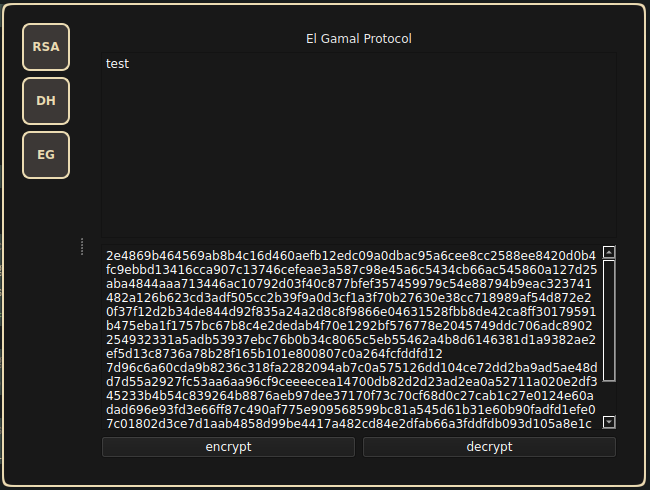
\includegraphics[width=0.48\textwidth]{res/png/02_elgamal_encryption.png}\label{fig:sub1}}
    \hfill
    \subfloat[Decryption]{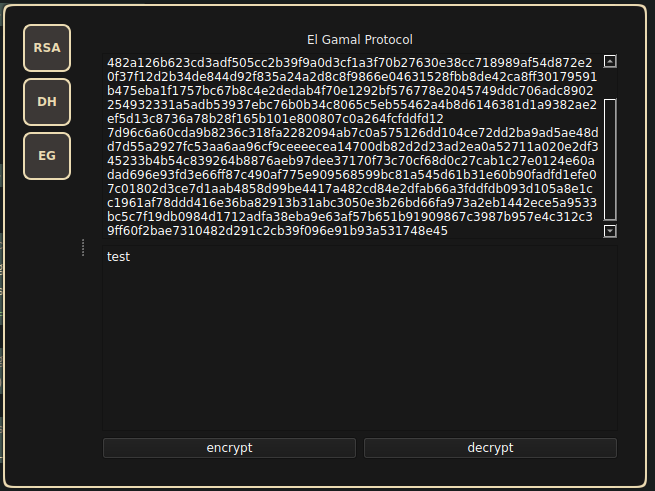
\includegraphics[width=0.48\textwidth]{res/png/03_elgamal_decryption.png}\label{fig:sub2}}
    \label{fig:side_by_side}
\end{figure}